% \begin{frame}
% 	\frametitle{Wirkungsquerschnitt}
% 	\begin{figure}
% 	\begin{center}
% 	  \includegraphics[width=0.3\textwidth]{../img/atlas_higgs_event.png}
% 	  \caption{Produkte einer Proton-Proton-Kollision beim ATLAS-Experiment am CERN (Quelle: https://cds.cern.ch/record/1459496)}
% 	\end{center}
% 	\end{figure}
% 	\begin{itemize}
% 		\item Bei Streuprozessen ist der Endzustand nicht eindeutig bestimmt
% 		\item Der Wahrscheinlichkeit eines bestimmten Endzustandes wird durch den Wirkungsquerschnitt $\sigma$ beschrieben.
% 		\item Differentieller Wirkungsquerschnitt $\frac{\difd \sigma}{\difd O}$ in Bezug auf \\
% 			  Observable $O$ (z.B. Raumwinkel $\Omega$, Transversalimpuls $p_\text{T}, \ldots$)
% 	\end{itemize}
% \end{frame}

\section{Theoretische Grundlagen}

\subsection{Das Standardmodell}
 \begin{frame}
 	\frametitle{Das Standardmodell}
 	\begin{figure}
 	\begin{center}
 	  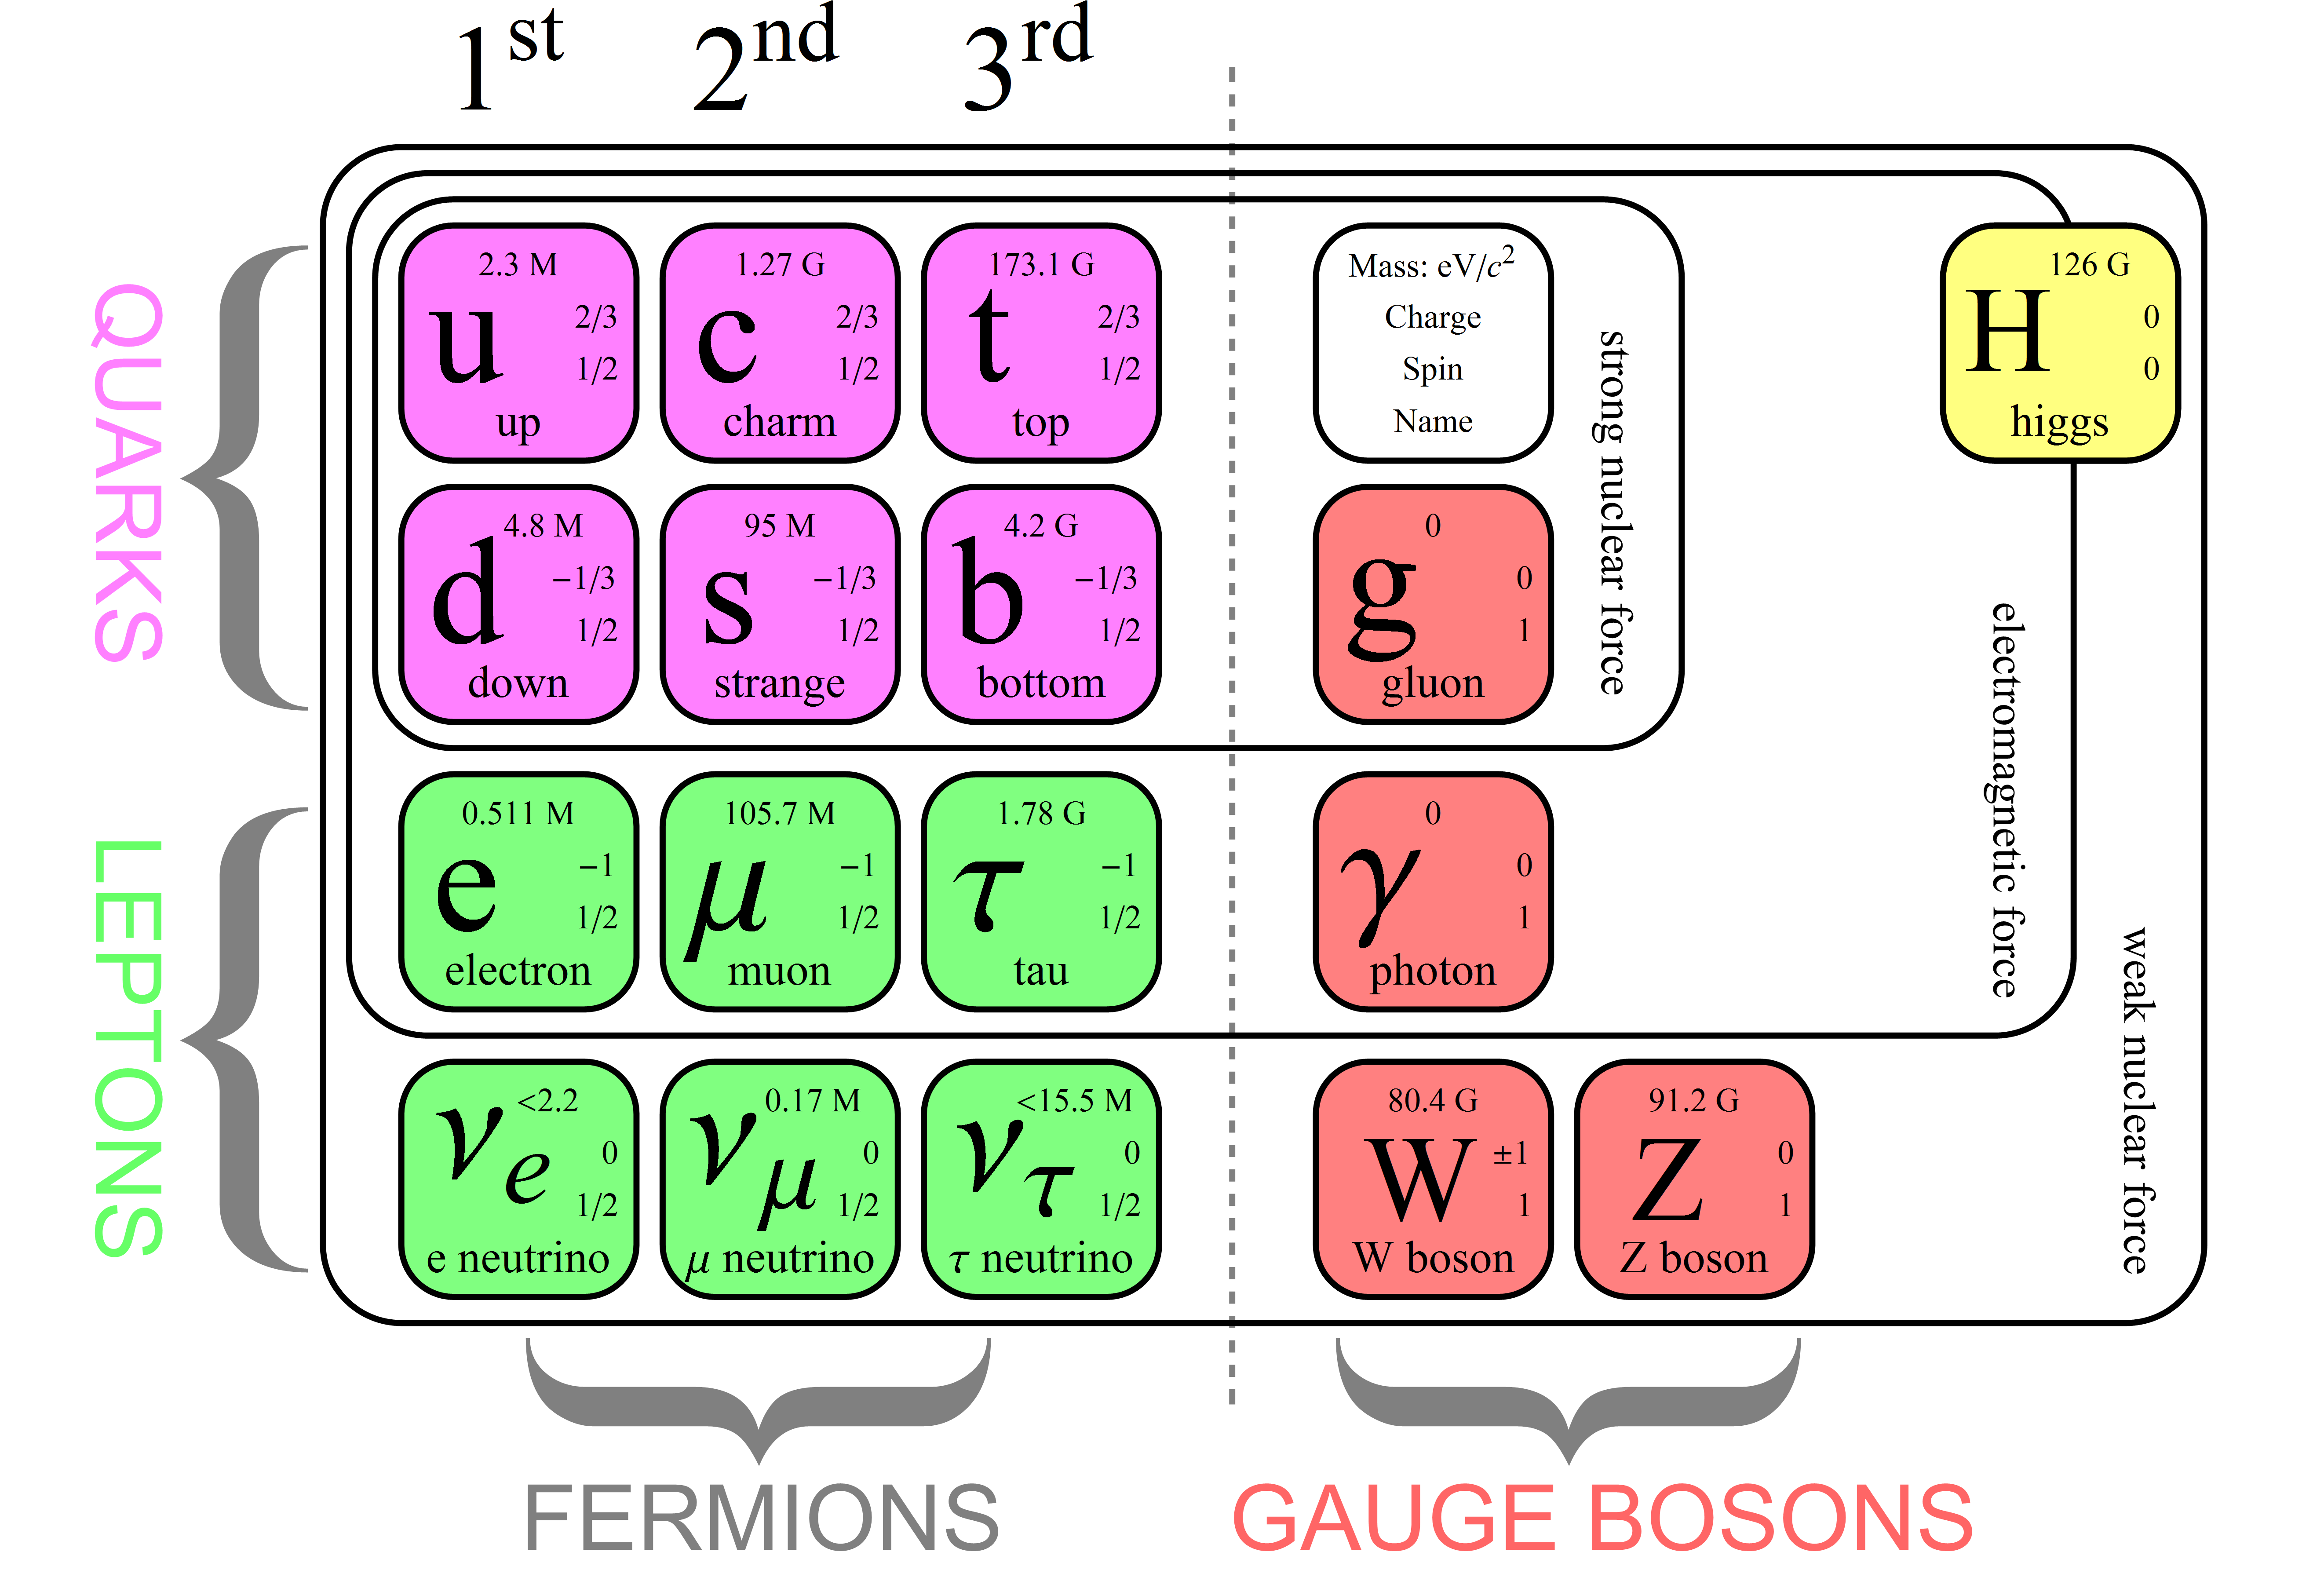
\includegraphics[width=0.9\textwidth]{graphics/SM1.png}
 	\end{center}
	\end{figure}
 \end{frame}
\begin{frame}
	\frametitle{Elektroschwache Wechselwirkung}
	\begin{center}
%		\begin{itemize}
%			\item
%			Bei hohen Energien haben elektromagnetische und schwache WW ähnliche Kopplungsstärken.
%			\item
%			Vereinheitlichung der Theorien durch Glasgow Salam und Weinberg
%			\item
%			Einführung der Bosonen $W^1$, $W^2$, $W^3$ und $B^0$ mit Physikalische Zuständen als Linearkombinationen
%		\end{itemize}
%		\begin{equation*}
%		\ket{W^{\pm}}=(1/\sqrt{2}) (\ket{W^1}\mp i\ket{W^2})
%		\end{equation*}
		\begin{equation*}
			\ket{\gamma} =  cos(\theta_w)\ket{B^0} + sin(\theta_w) \ket{W^3}
		\end{equation*}
		\begin{equation*}
		\ket{Z^0} = -sin(\theta_w) \ket{B^0} + cos(\theta_w) \ket{W^3}
		\end{equation*}\\
		\begin{equation*}
		\textcolor{lightgray}{sin^2(\theta_w)\cdot cos^2(\theta_w) = \frac{\pi\alpha}{\sqrt{2}G_FM_Z^2}}
		\end{equation*}
		\begin{equation*}
		\textcolor{lightgray}{M_W = M_Z~cos(\theta_w)}
		\end{equation*}
		\begin{equation*}
		\textcolor{lightgray}{g_V^f = I^f_3-2 Q_f sin^2(\theta_w)}
		\end{equation*}
		\begin{equation*}
		\textcolor{lightgray}{g_A^f = I^f_3}
		\end{equation*}
	\end{center}
\end{frame}
\begin{frame}
	\frametitle{Elektroschwache Wechselwirkung}
	\begin{center}
		\begin{equation*}
		\textcolor{lightgray}{\ket{\gamma} =  cos(\theta_w)\ket{B^0} + sin(\theta_w) \ket{W^3}}
		\end{equation*}
		\begin{equation*}
		\textcolor{lightgray}{\ket{Z^0} = -sin(\theta_w) \ket{B^0} + cos(\theta_w) \ket{W^3}}
		\end{equation*}
		\\
		\begin{equation*}
		sin^2(\theta_w)\cdot cos^2(\theta_w) = \frac{\pi\alpha}{\sqrt{2}G_FM_Z^2}
		\end{equation*}
		\begin{equation*}
		M_W = M_Z~cos(\theta_w)
		\end{equation*}
		\begin{equation*}
			\textcolor{lightgray}{g_V^f = I^f_3-2 Q_f sin^2(\theta_w)}
		\end{equation*}
		\begin{equation*}
			\textcolor{lightgray}{g_A^f = I^f_3}
		\end{equation*}
	\end{center}
\end{frame}

\begin{frame}
	\frametitle{Elektroschwache Wechselwirkung}
	\begin{center}
		\begin{equation*}
		\textcolor{lightgray}{\ket{\gamma} =  cos(\theta_w)\ket{B^0} + sin(\theta_w) \ket{W^3}}
		\end{equation*}
		\begin{equation*}
		\textcolor{lightgray}{\ket{Z^0} = -sin(\theta_w) \ket{B^0} + cos(\theta_w) \ket{W^3}}
		\end{equation*}
		\\
		\begin{equation*}
		\textcolor{lightgray}{sin^2(\theta_w)\cdot cos^2(\theta_w) = \frac{\pi\alpha}{\sqrt{2}G_FM_Z^2}}
		\end{equation*}
		\begin{equation*}
		\textcolor{lightgray}{M_W = M_Z~cos(\theta_w)}
		\end{equation*}
		\begin{equation*}
		g_V^f = I^f_3-2 Q_f sin^2(\theta_w)
		\end{equation*}
		\begin{equation*}
		g_A^f = I^f_3
		\end{equation*}
	\end{center}
\end{frame}

\subsection{$e^+e^-$ Kollisionen}
\begin{frame}
	\frametitle{Annihilation $e^+e^- \rightarrow f\bar{f}$ }
	\begin{center}
		\begin{figure}
			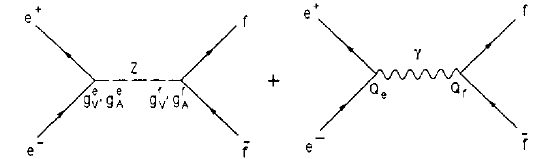
\includegraphics[width=1.0\textwidth]{graphics/annihilation.png}
		\end{figure}
	\end{center}
\end{frame}
\begin{frame}
	\frametitle{Bhabha Streuung $e^+e^- \rightarrow e^+e^-$ }
	\begin{center}
		\begin{figure}
			\includegraphics[width=0.8\textwidth]{graphics/Bhabbastreuung.png}
		\end{figure}
	\end{center}
	\begin{equation*}
	\frac{d\sigma_s}{d\Omega} \propto (1+cos^2(\theta)),\qquad\frac{d\sigma_t}{d\Omega} \propto (1-cos(\theta))^{-2}
	\end{equation*}
\end{frame}
\begin{frame}
	\frametitle{Strahlungskorrekturen}
	\begin{figure}
		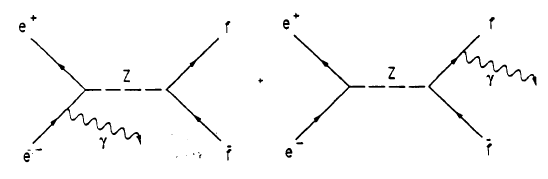
\includegraphics[width=0.75\linewidth]{graphics/Bremsstrahlungskorrektur}
	\end{figure}
	\begin{center}
	\begin{minipage}{0.4\linewidth}
			\begin{figure}
				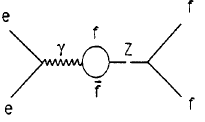
\includegraphics[width=0.8\linewidth]{graphics/presentationvertexschleifen}
			\end{figure}
	\end{minipage}
	\begin{minipage}{0.4\linewidth}
	\begin{figure}
			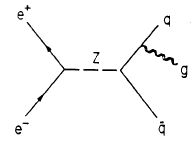
\includegraphics[width=0.8\linewidth]{graphics/presentation_QCDkorrektur}
	\end{figure}
	\end{minipage}
	\end{center}
\end{frame}

\subsection{Wirkungsquerschnitt und Zerfallsbreite}
\begin{frame}
	\frametitle{Wirkungsquerschnitt}
	\hspace{1cm} Ereignisrate bei Luminosität $L$:
	\begin{equation*}
	\scalebox{1.5}{$\dot{N} = \sigma \cdot L$}
	\end{equation*}
	\hspace{1cm} Wirkungsquerschnitt messen:
	\begin{equation*}
	\scalebox{1.5}{$\sigma = \frac{N}{\int L~\text{d}t}$}
	\end{equation*}
\end{frame}
\begin{frame}
	\frametitle{Zerfallsbreite}
	\hspace{1cm} Energieunschärfe:
	\begin{equation*}
	\hbar=T_Z\cdot\Gamma_Z
	\end{equation*}
	\hspace{1cm} Gesamtzerfallsbreite:
	\begin{equation*}
	\Gamma_Z = \Gamma_e+ \Gamma_{\mu} + \Gamma_{\tau} + 3 \cdot \Gamma_{\nu}
	\end{equation*}
\end{frame}

\begin{frame}
	\frametitle{Schwerpunktsenergie und Wirkungsquerschnitt}
	\begin{equation*}
	\sigma(s) = \frac{12\pi}{ \tikzmark{MZ1}M_Z^2}
	\frac{s\tikzmark{gammae}\Gamma_e \tikzmark{gammaf}\Gamma_f}{(s-\tikzmark{MZ2}M_Z^2)^2 + s^2\cdot\tikzmark{gammaZ}\Gamma_Z^2 / \tikzmark{MZ3}M_Z^2}
	\end{equation*}
	\begin{tikzpicture}[
	remember picture,
	overlay,
	expl1/.style={draw=orange,fill=orange!30,rounded corners},
	expl2/.style={draw=gray!20,fill=gray!10,rounded corners},
	arrow1/.style={red!80!black,ultra thick,->,>=latex},
	arrow2/.style={gray!20,ultra thick,->,>=latex}
	]
	\node[expl1]
	(gammaeexpl)
	at (2,2cm)
	{\textcolor{black}{Zerfallsbreite Elektron}};
	\node[expl1]
	(gammafexpl)
	at (10,2cm)
	{\textcolor{black}{Zerfallsbreite Fermion}};
	\node[expl1]
	(MZexpl)
	at (1,-1cm)
	{Masse $Z^0$};
	\node[expl1]
	(gammaZexpl)
	at (9.8,-1cm)
	{\textcolor{black}{Gesamtzerfallsbreite $Z^0$}};
	\draw[arrow1]
	(gammafexpl.west) to[out=180,in=90] ([yshift=-8.2ex,xshift=1.5ex]{pic cs:gammaf});
	\draw[arrow1]
	(gammaeexpl.east) to[out=0,in=90] ([yshift=2ex,xshift=0.5ex]{pic cs:gammae});
	\draw[arrow1]
	(gammaZexpl.west) to[out=180,in=270] ([yshift=-10.5ex,xshift=0.5ex]{pic cs:gammaZ});
	\draw[arrow1]
	(MZexpl.east) to[out=0,in=270] ([yshift=-10.5ex,xshift=1ex]{pic cs:MZ1});
	%\draw[arrow1]
	%(MZexpl.east) to[out=0,in=270] ([yshift=-10.5ex,xshift=1ex]{pic cs:MZ2});
	%\draw[arrow1]
	%(MZexpl.east) to[out=0,in=270] ([yshift=-10.5ex,xshift=1ex]{pic cs:MZ3});
	\end{tikzpicture}
\end{frame}
\subsection{Vorwärts Rückwärts Asymmetrie}
\begin{frame}
	\frametitle{Vorwärts Rückwärts Asymmetrie}
	\begin{center}
		\begin{equation*}
		\sigma_f=\int_{0}^{1}\frac{\text{d}\sigma}{\text{d}cos(\theta)}~\text{d}cos(\theta)
		\end{equation*}
		\begin{equation*}
		\sigma_b=\int_{-1}^{0}\frac{\text{d}\sigma}{\text{d}cos(\theta)}~\text{d}cos(\theta)
		\end{equation*}
		\\
		\begin{equation*}
		\textcolor{lightgray}{A_{fb}=\frac{\sigma_f-\sigma_b}{\sigma_f+\sigma_b}}
		\end{equation*}
	\end{center}
\end{frame}
\begin{frame}
	\frametitle{Vorwärts Rückwärts Asymmetrie}
	\begin{center}
		\begin{equation*}
		\textcolor{lightgray}{\sigma_f=\int_{0}^{1}\frac{\text{d}\sigma}{\text{d}cos(\theta)}~\text{d}cos(\theta)}
		\end{equation*}
		\begin{equation*}
		\textcolor{lightgray}{\sigma_b=\int_{-1}^{0}\frac{\text{d}\sigma}{\text{d}cos(\theta)}~\text{d}cos(\theta)}
		\end{equation*}
		\\
		\begin{equation*}
		A_{fb}=\frac{\sigma_f-\sigma_b}{\sigma_f+\sigma_b}
		\end{equation*}
	\end{center}
\end{frame}
\begin{frame}
	\frametitle{Vorwärts Rückwärts Asymmetrie}
	\begin{center}
		Für Leptonen am Resonanzpeak:
		\begin{equation*}
		A_{fb}^{\ell,peak}\approx 3 \left ( \frac{g^{\ell}_V}{g^{\ell}_A} \right )^2=3\cdot (1-4 sin^2(\theta_w))
		\end{equation*}
	\end{center}
\end{frame}